%
% IMPORTANT: THIS TEMPLATE NEEDS TO BE COMPILED WITH XeLaTeX
%
% This template uses several fonts not included with Windows/Linux by
% default. If you get compilation errors saying a font is missing, find the line
% on which the font is used and either change it to a font included with your
% operating system or comment the line out to use the default font.
%


\documentclass[letterpaper, article]{deedy-resume-openfont}


\begin{document}

%%%%%%%%%%%%%%%%%%%%%%%%%%%%%%%%%%%%%%
%
%     TITLE NAME
%
%%%%%%%%%%%%%%%%%%%%%%%%%%%%%%%%%%%%%%


\namesection{Aaron}{Wubshet}
{ 404.563.9110 | awubshet@mit.edu | www.github.com/aaronwubshet | www.linkedin.com/in/aaronwubshet}

%%%%%%%%%%%%%%%%%%%%%%%%%%%%%%%%%%%%%%
%
%     COLUMN ONE
%
%%%%%%%%%%%%%%%%%%%%%%%%%%%%%%%%%%%%%%
\hfill

\begin{minipage}[t]{0.66\textwidth}
%%%%%%%%%%%%%%%%%%%%%%%%%%%%%%%%%%%%%%
%     EXPERIENCE
%%%%%%%%%%%%%%%%%%%%%%%%%%%%%%%%%%%%%%
\vspace{.01cm}
\section{Experience}

% \runsubsection{Bain \& Company}
% \descript{| Associate Consultant Intern}
% \location{Jun - Aug 2018 | Atlanta, GA}
% \vspace{\topsep} % Hacky fix for awkward extra vertical space
% \begin{tightemize}
% 	\item Crash course into management and strategy consulting with seminars on Bain
% 	\item Worked alongside a Bain case team to help a client develop their corporate venture capital business unit
% \end{tightemize}
% \sectionsep

\runsubsection{HK Innovation Node}
\descript{| Entrepreneur \& Maker Intern}
\location{Jan 2018 | Kowloon Tong, Hong Kong}
\vspace{\topsep} % Hacky fix for awkward extra vertical space
\begin{tightemize}
	\item MIT-Hong Kong integrator for entrepreneurship \& hardware start ups
	\item Worked with a diverse team of engineers and designers to create TrueLink, a module designed to evoke emotion from loved ones over long distances.
\end{tightemize}
\sectionsep

\runsubsection{Draper}
\descript{| Signal Engineering Intern }
\location{Jan 2017 \& June - Aug 2017 | Cambridge, MA}
\begin{tightemize}
	\item Created GSM network via GNU Radio \& universal software radio peripherals
	\item Developed novel MatLab simulator for aggregate LTE power levels
\end{tightemize}
\sectionsep

\runsubsection{Bain \& Company}
\descript{| Building Entrepreneurial Leaders}
\location{Aug 2017 | Atlanta, GA}
\begin{tightemize}
	\item Preview of strategic management consulting with seminars on Bain work flow
	\item Designed a strategy for developing a client's venture capital business unit
\end{tightemize}
\sectionsep

\runsubsection{MIT Consulting Group}
\descript{| CFO \& Case Team Leader}
\location{Feb 2016 – Present | Cambridge, MA}
\begin{tightemize}
	\item Managed a yearly budget of approximately \$ 50,000 as treasurer while providing clients with a wide array of consulting services
	\item Clients range from big tech to start-ups to government agencies with cases of prototyping, market penetration strategies, and partnership evaluation
\end{tightemize}
\sectionsep

\runsubsection{MIT EECS \& Physics}
\descript{| Teaching and Grading Faculty }
\location{Feb 2016 – Present | Cambridge, MA}
\begin{tightemize}
	\item Member of the teaching staff for classes in the physics and EECS department
	\item Classes ranged from Circuit Design to Feedback Systems to E\&M Physics
\end{tightemize}
\sectionsep

\runsubsection{MIT MakerLodge}
\descript{| Electronics Team Lead \& PR Chair}
\location{Feb 2017 – Aug 2017 | Cambridge, MA}
\begin{tightemize}
	\item Co-head of the electronics training team and public relations chair
	\item Designed electronics training and fostered relations with MIT community
\end{tightemize}

%%%%%%%%%%%%%%%%%%%%%%%%%%%%%%%%%%%%%%%
%%    CLASS Projects
%%%%%%%%%%%%%%%%%%%%%%%%%%%%%%%%%%%%%%%

\section{Class Projects}
\runsubsection{A Drone's Eye View: Engineering Interactive Tech}
\\
\location{Sept - Dec 2017 | Cambridge, MA}
\begin{tightemize}
	\item Drone mounted projector system to turn any surface into an interactive experience with leap motion gesture recognition
	\item Incorporated OptiTrack IR Tracking system, microcomputer programming, and leap motion gesture recognition to create mobile interface system
\end{tightemize}

\runsubsection{Speaker Tracking: Microcomputer Laboratory}
\\
\location{Apr - May 2017 | Cambridge, MA}
\begin{tightemize}
	\item Created a target following speaker system that turned to face the target, automatically adjusting volume as needed
	\item Designed the system using the Intel 8051 microcontroller and Cypress PSoC
\end{tightemize}

\runsubsection{Audio Noise Cancellation}
\\
\location{Mar - Apr 2017 | Cambridge, MA}
\begin{tightemize}
	\item Designed a feedback based noise cancellation system with custom enclosure
	\item Built circuitry to recreate the simulation results on the physical speaker
\end{tightemize}

\end{minipage}
\hfill
%%%%%%%%%%%%%%%%%%%%%%%%%%%%%%%%%%%%%%
%
%     COLUMN TWO
%
%%%%%%%%%%%%%%%%%%%%%%%%%%%%%%%%%%%%%%
\begin{minipage}[t]{0.33\textwidth}

%%%%%%%%%%%%%%%%%%%%%%%%%%%%%%%%%%%%%%
%     EDUCATION
%%%%%%%%%%%%%%%%%%%%%%%%%%%%%%%%%%%%%%
\vspace{\topsep}
\centering{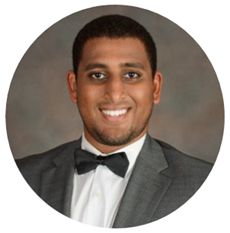
\includegraphics{resume_image.PNG}}


\section{Education}

\subsection{Massachusetts Institute \hfill}
\subsection{of Technology \hfill}
\descript{{\large BS in Electrical Engineering}}
\location{June 2019 | Cambridge, MA \\ GPA: 4.4}
\sectionsep

\subsection{Relevant Coursework \hfill}
\vspace{.05cm}
6.302: Feedback Systems and Controls\\
6.111: Digital Systems Laboratory \\
6.175: Computer Architecture


%%%%%%%%%%%%%%%%%%%%%%%%%%%%%%%%%%%%%
%     SKILLS
%%%%%%%%%%%%%%%%%%%%%%%%%%%%%%%%%%%%%%

\section{Skills}
\subsection{Technical}

Verilog/BSV \hspace{2.625cm} \textbullet \textbullet  \textbullet \textbullet \textbullet \\
MatLab \hspace{3.28cm} \textbullet \textbullet \textbullet \textbullet  \textbullet\\
Eagle/Altium \hspace{2.53cm} \textbullet \textbullet \textbullet \textbullet \\
Python \hspace{3.37cm}  \textbullet \textbullet  \textbullet \\

\sectionsep

\subsection{Management}
Accounting \hspace{2.75cm} \textbullet \textbullet \textbullet  \textbullet \textbullet\\
Logistics \hspace{3.15cm} \textbullet \textbullet  \textbullet \textbullet \\
Resource Allocation \hspace{1.47cm} \textbullet \textbullet \textbullet \textbullet \\

%%%%%%%%%%%%%%%%%%%%%%%%%%%%%%%%%%%%%
%     PERSONAL PROJECTS
%%%%%%%%%%%%%%%%%%%%%%%%%%%%%%%%%%%%%%
\section{Personal Projects}

\subsection{SSL/STAR Labs \hfill}
Designed and implemented circuitry \& control software for a CubeSat project
 \sectionsep
\subsection{RLE@MIT\hfill}
Experimentalist creating transparent displays with nanoparticles dispersed in polymer matrix.
 \sectionsep
\subsection{Movie Rating WebApp\hfill}
Social multimedia platform with a feedback based value system for movie choices
\sectionsep
\subsection{Quantum Chemistry@GT\hfill}
Experimentalist designing laser modulation system to ion trap Ca\textsuperscript{2+}

\end{minipage}

\end{document}
